\documentclass[sigchi]{acmart}

\def\tightlist{}
\settopmatter{printacmref=false}
\renewcommand\footnotetextcopyrightpermission[1]{}

\usepackage{booktabs} % For formal tables

% Copyright
\setcopyright{none}
%\setcopyright{acmcopyright}
%\setcopyright{acmlicensed}
%\setcopyright{rightsretained}
%\setcopyright{usgov}
%\setcopyright{usgovmixed}
%\setcopyright{cagov}
%\setcopyright{licensedcagov}
%\setcopyright{cagovmixed}
%\setcopyright{licensedothergov}

% DOI
\acmDOI{10.475/123_4}

% ISBN
\acmISBN{123-4567-24-567/08/06}

%Conference
\acmConference[Business Intelligence]{Assignment 3}{January 2021}{Linz/Vienna, Austria}
\acmYear{2021}
\copyrightyear{2021}

\acmPrice{15.00}


\begin{document}
\title{Predicting the resale value of used cars}
\subtitle{Created using R Markdown}

\author{Simone Andreetto}
\affiliation{%
  \institution{01635069}
}

\author{Felix Winterleitner}
\affiliation{%
  \institution{01612776}
}

% The default list of authors is too long for headers.
\renewcommand{\shortauthors}{S. Andreetto et al.}


\begin{abstract}
This is Assignment 3 in Business Intelligence @ TU Wien in the winter term of 2020.
\end{abstract}


\keywords{Business Intelligence, R, Rmd, Spark}

\begin{teaserfigure}
  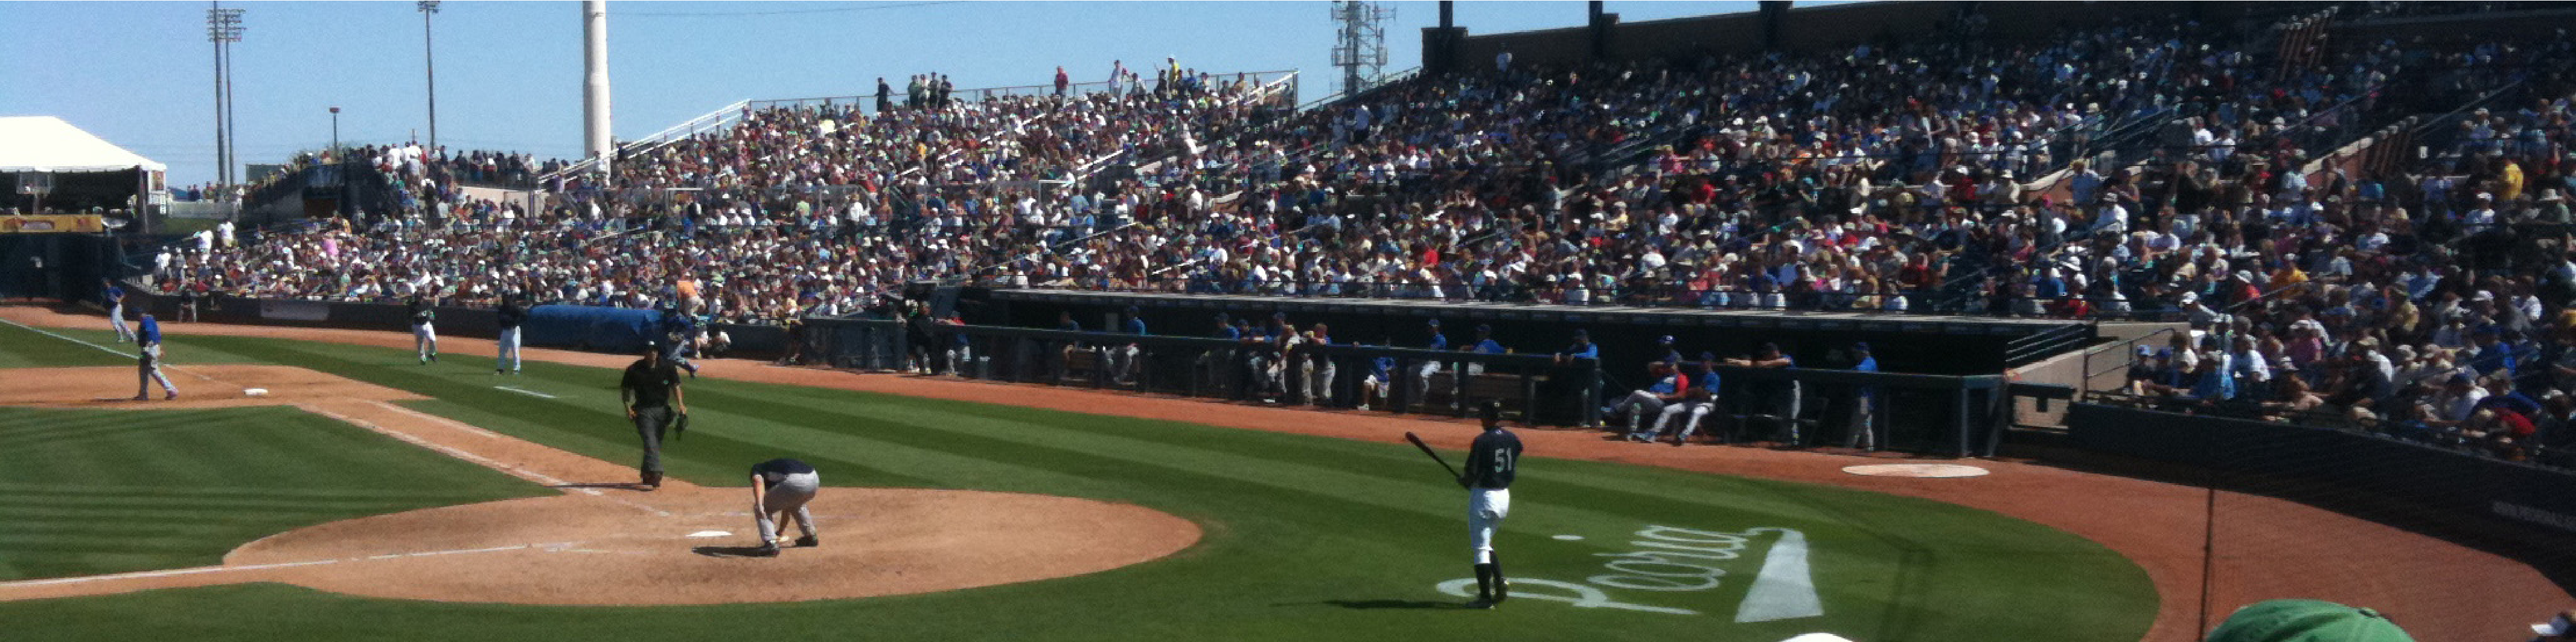
\includegraphics[width=\textwidth]{sampleteaser}
  \caption{This is a teaser}
  \label{fig:teaser}
\end{teaserfigure}


\maketitle

\hypertarget{introduction}{%
\section{Introduction}\label{introduction}}

For this project, we used a dataset found on Kaggle.com provided by user Aditya \citep{Aditya}. It contains a collection of different used car listings obtained by searching through online marketplaces using a web scraper. The dataset is split into different files, one per car brand. The brands for which data is available are:

\begin{itemize}
\tightlist
\item
  Audi
\item
  BMW
\end{itemize}

\hypertarget{history}{%
\section{History}\label{history}}

Tribute was the first song Black and Gass played live as Tenacious D. The song, like many other songs that were recorded on Tenacious D, was originally performed on their short-lived HBO TV series. During earlier performances of this song Kyle Gass played the opening to ``Stairway to Heaven''. The two songs are both in A minor and have very similar chord progressions, and critics have said the songs sound alike.\citep{Cowan1988, Gluck2005, Wardak2002} \textbf{The maturation of the song over time is shown in Figure \ref{fig:tribute-plot}.}

\begin{figure}
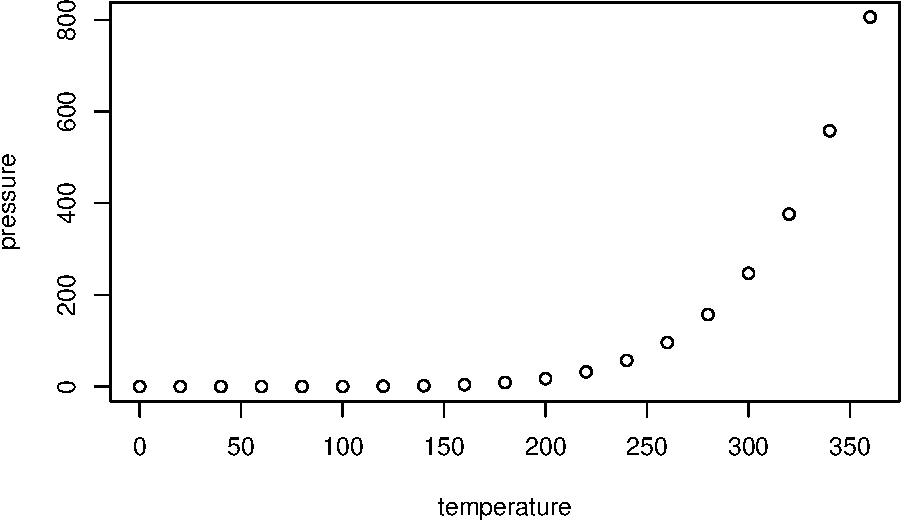
\includegraphics[width=0.98\columnwidth]{step6_files/figure-latex/tribute-plot-1} \caption{This is how great Tribute gets over time}\label{fig:tribute-plot}
\end{figure}

\begin{figure*}
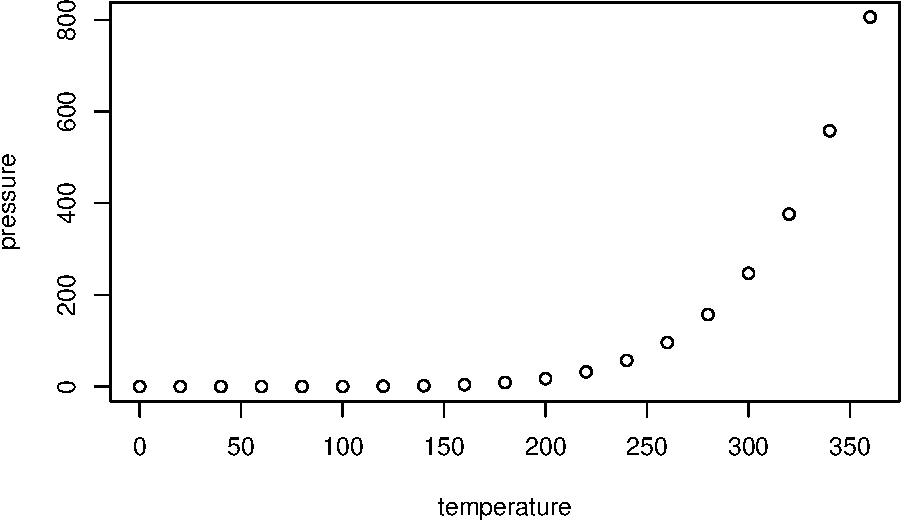
\includegraphics[width=0.98\textwidth]{step6_files/figure-latex/two-col-tribute-plot-1} \caption{This is a two-column plot of how great Tribute gets over time}\label{fig:two-col-tribute-plot}
\end{figure*}

\hypertarget{synopsis}{%
\subsection{Synopsis}\label{synopsis}}

The song chronicles the band members' encounter with a demon who demands the duo play ``the best song in the world'' or have their souls eaten. Having nothing to lose from trying, they play ``the first thing that came to our heads'', and it ``just so happened to be the best song in the world.''\citep{Wardak2002}

\begin{table}

\caption{\label{tab:table-iris}The favorite iris' of Tenacious D.}
\centering
\begin{tabular}[t]{rrrr}
\toprule
Sepal.Length & Sepal.Width & Petal.Length & Petal.Width\\
\midrule
5.1 & 3.5 & 1.4 & 0.2\\
4.9 & 3.0 & 1.4 & 0.2\\
4.7 & 3.2 & 1.3 & 0.2\\
4.6 & 3.1 & 1.5 & 0.2\\
5.0 & 3.6 & 1.4 & 0.2\\
\addlinespace
5.4 & 3.9 & 1.7 & 0.4\\
4.6 & 3.4 & 1.4 & 0.3\\
5.0 & 3.4 & 1.5 & 0.2\\
4.4 & 2.9 & 1.4 & 0.2\\
4.9 & 3.1 & 1.5 & 0.1\\
\bottomrule
\end{tabular}
\end{table}

Given the ``Stairway to Heaven'' interlude in the original TV series version, along with the similarity of the chord progression in both songs, Tribute at first implies that the best song in the world is indeed that song. However, the lyrics make clear that Tribute sounds nothing like the song they came up with to please the demon; as Black describes: ``And the peculiar thing is this my friends: The song we sang on that fateful night, it didn't actually sound anything like this song.''

\bibliographystyle{ACM-Reference-Format}
\bibliography{my-bibliography}

\end{document}
